\section{Intelligence}
\begin{itemize}
    \item \emph{The ability to acquire and apply knowledge and skills, the faculty of understanding} (Dictionaries)
    \item \emph{The ability to achieve complex goals} (Max Tegmark, Life 3.0)
    \begin{itemize}
        \item This inherently implies the first definition
    \end{itemize}
\end{itemize}

According to the second definition, it should be possible to have different levels of intelligence based on the complex goals achieved. e.g. winning tic-tac-toe as opposed to chess. However, we then run into the problem of not all goals being equal - certain agents are naturally better at certain tasks than others. e.g. judging a fish to climb a tree

\subsection{Perspectives on Intelligence}

\subsubsection{Anthropomorphic Perspective}
According to humans, identifying someone in a photo is much easier than performing complicated multiplication: but it's the opposite to a computer.\\

\emph{Moravec's Paradox} is that certain tasks (such as low level sensorimotor like walking/judging depth) are very easy to humans, but are actually incredibly complex to replicate, as we're discovering by trying to build machines that can do the same. Humans feel that these tasks are easy because we have specialised dedicated hardware that has evolved to achieve them. 

\subsubsection{Machine/AI Perspective}
Intelligence is entirely based on information storage/retrieval and computation - this makes no reference to having organic matter (i.e. a brain), and thus eventually a machine could become intelligent. This approach believes that intelligence is \emph{substrate neutral}.

\subsection{Requirements}

\subsubsection{Information Storage}
Information storage devices arrange into particular states to represent some information - these states must be stable enough that a random disturbance (at an atomic level) can't change them. e.g. magnetising 0s and 1s onto a surface\\

Information storage is substrate neutral: human brains store information electrically (neurons firing) and chemically (strength of synapses in the brain), while large computers can have more storage than a brain. Information retrieval in computers is address-based, while in brains it's association-based (similar information is stored together).

\subsubsection{Computation}
Using a function to transform one information state into another - the more complex the function, the more complex the achieved goals. Functions/dynamics must be predictable and stable: if given an input, the output is the desired function of the input.\\

Computation is substrate neutral - anything that can replicate a turing machine can perform any well formed function (e.g. NAND gates, Magic the Gathering cards). Any universally intelligent machine with the time, resources and \emph{motivation}, can improve itself to be able to solve any goals as well as a superintelligent machine. 

\subsection{Agent Approach to AI}
To achieve complex goals, intelligence requires action (talking/speaking is an action), simply deliberating isn't enough. \emph{Russell and Norvig} favour an rational-acting approach to AI, as opposed to not effecting and just thinking rationally, or acting/thinking like humans. \\

They posit that AI is the field of building intelligent agents, which take in perceptions and output behaviour based on these.

\subsubsection{Ideal Agents}
A perfectly rational agent that models the environment, considers actions and their expected utilities (utility of resulting state X probability of achieving that state), and chooses the action with the highest expected utility. \\

It's not possible to build a \emph{perfectly} rational agent, or if it is it's not possible to perfectly implement it - this is because by the time the agent deliberates on the most rational action for an environment, the environment would have changed.\\

An agent is \emph{calculative rational} if it's behaviour would be perfect if executed infinitely fast (i.e.$time_{deliberation} \rightarrow 0$). \emph{Bounded Optimality} is the most optimal agent given the machine and the environment.

\subsubsection{Universal AI (AIXI)}Intelligence is defined as the agent's ability able to achieve goals in a wide range of environments (Shane Legg/Marcus Hutter). AIXI is a mathematical framework that turns this definition into 'reality' to define a perfect agent. \\
It's not possible to build such an agent, as it requires infinite processing power: instead, we can use it as an aim for how a perfect AI should be able to act.

\subsection{Artificial General Intelligence}

\subsubsection{AGI vs Narrow AI}
\begin{description}
\item[Narrow AI] AI built for a a specific task. e.g. Alpha Go, Hawkeye, Facial recognition systems
\item[Artificial General Intelligence] Can achieve any goal as well as humans, and possesses: common sense, the ability to learn and reason, process complex information across multiple domains
\end{description}



\subsubsection{Moravec's Landscape of Human Competence and the Singularity}
\begin{figure}[H]
    \centering
    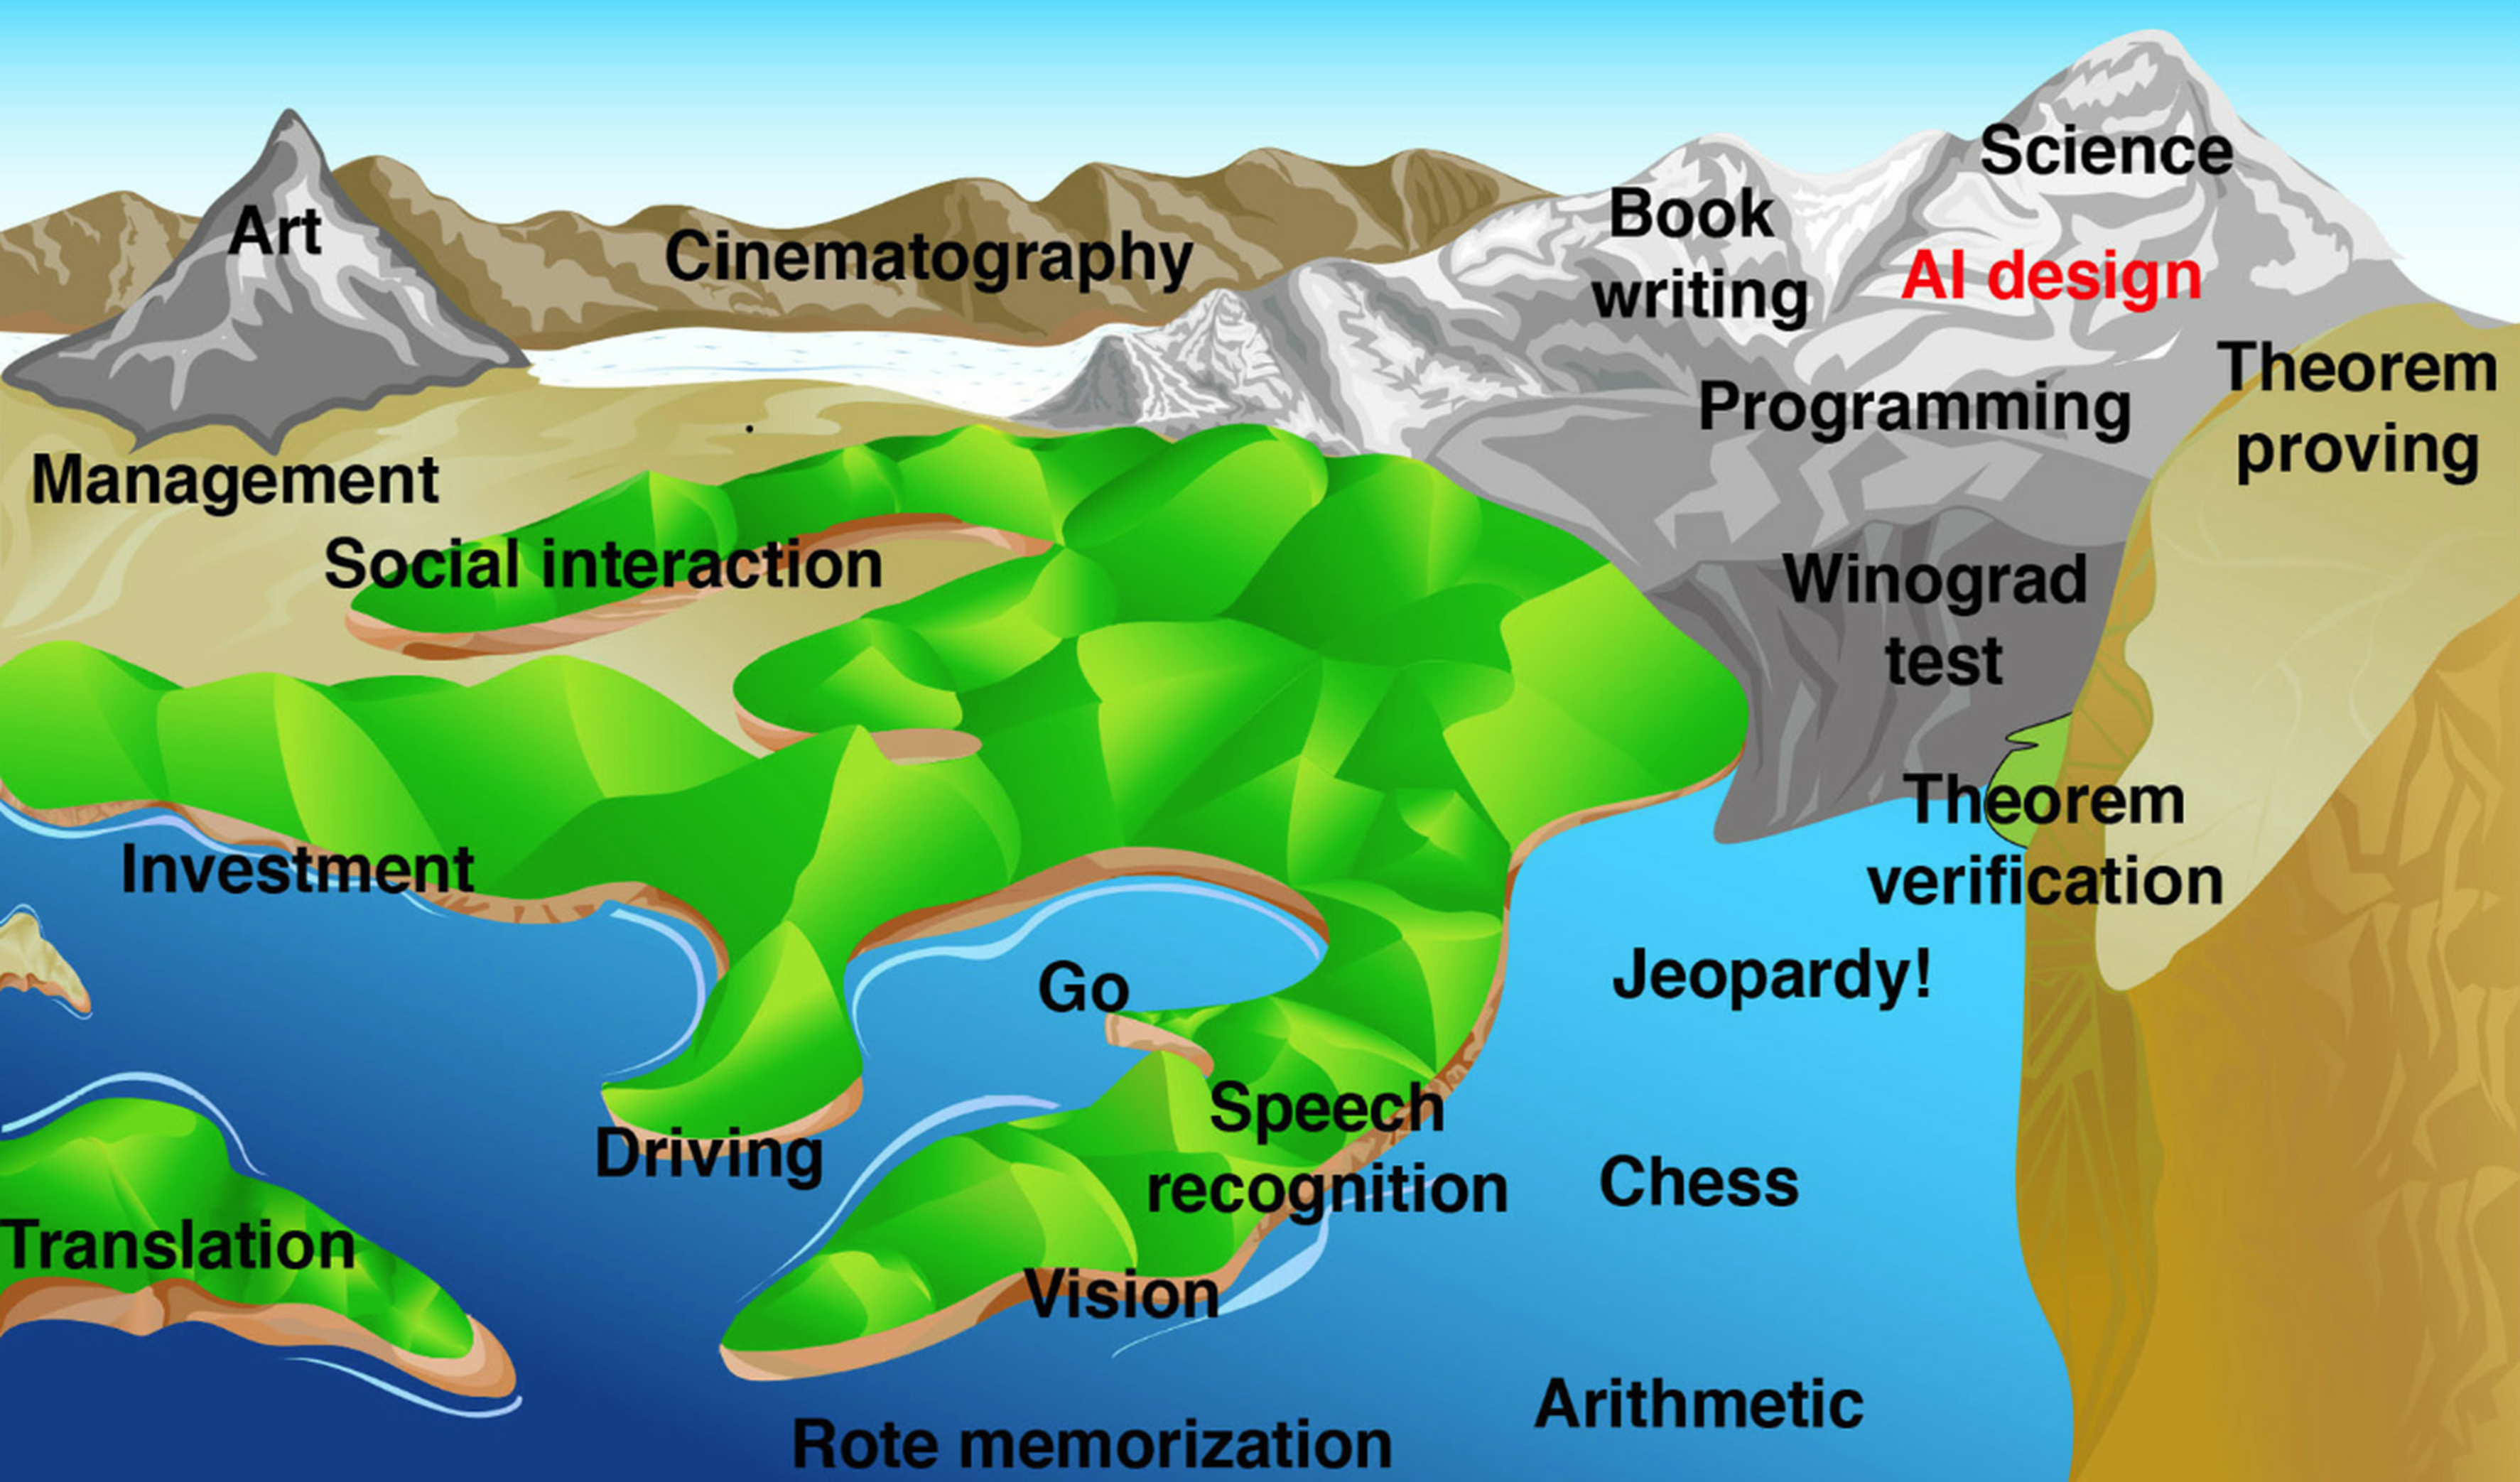
\includegraphics[width = \textwidth, height=7cm,keepaspectratio ]{Images/landscape-of-human-competence}
\end{figure}
The above image (from 1998) shows various fields of human achievement, and the water level shows AI's current level of competence in these fields. An AI that is able to achieve all of these is an AGI, however an AI learns how to design AI will be able to design an AGI infinitely faster than a human.\\

Such an event is a \emph{Singularity} - AI will be faster at designing AI than us, and can thus reach newer levels of intelligence that we can't currently comprehend - this \emph{Superintelligence} (exceeds humans' cognitive performance in all relavant areas) will be to humans as humans are to animals. 

\subsubsection{Paths to AGI}
\begin{enumerate}
    \item Good Old Fashioned AI - logic/symbol paradigms - highly brittle, subject to initial assumptions/axioms, difficult to translate the world into symbols
    \item Machine Learning - learns like humans do, less susceptible to false data as it slowly degrades - backpropogation algorithms + advances in hardware have made neural nets very popular \\ \quad \quad - Alan Turing also suggested ML, to build a system that simulates a child's brain then give it data to learn from
\end{enumerate}

\subsubsection{How long till AGI?}
According to a survey of experts in \emph{Superintellgence} (by Nick Bostrom), AGI will be achieved in 20 years (the same estimate was made in 1940). After that, superintelligence will be achieved within 30 years.\\

AGI/Superintelligence will change the role of humans on the planet irreversibly, so it's best to estimate and prepare for their impact before it actually happens. 

\subsection{Turing Test}

\subsubsection{Recognising AGI}
Common sense and Natural Language understanding are AI-complete problems: as hard to solve as AGI. Therefore, being able to understand/synthesise natural language is a strong indicator of intelligence. Decartes in 1669 said that a machine would never be able to produce a meaningful arrangement of words.

\subsubsection{Format of the Test}
A human and a computer both independently talk to a judge, who can ask them questions. If the judge can't do better than a 50/50 guess on which is which based on the answers, the computer has passed, and is able to \emph{act like a human}.\\

Note this doesn't coincide with the usual definition of being able to act rationally. 

\subsubsection{Logical Sufficiency/Necessity}
\begin{description}
    \item[Logical Sufficiency] Pass the Turing test $\rightarrow$ Intelligence \\ \quad for $x\rightarrow Y$, x is enough to prove y. 
    \item[Logical Necessity] Intelligence $\rightarrow$ Pass the Turing Test \\ \quad for $y\rightarrow x$, y can't be true without x
\end{description}
By definition, $A\rightarrow B$ implies B can be true without B.

\begin{enumerate}
    \item Pass $\leftrightarrow$ Intelligence : few people agree on this, as it means intelligent creatures without the same type of language wouldn't pass (\emph{chauvinistic objection})
    
    \item Pass $\rightarrow$ Intelligence : Logically impossible that if an agent passes the test, it's not intelligent. However, a perfect lookup table of responses could pass (e.g. Searle's Chinese room) - this doesn't use intelligence, it simply reads the table. Arguments against this say such a lookup table isn't logically possible (though it's conceivable), or that such an agent is intelligent (processes information and produces behaviour like a human)
    
    \item Intelligence $\rightarrow Pass$ : Everything with intelligence MUST pass the test, but things can pass without intelligence. Similar to 1, there may be intelligence that doesn't have the same language conventions
\end{enumerate}

\subsubsection{Results and Responses}
Though the test isn't perfect, it gives a strong probability of intelligence - the original paper mentioned that an 'average' interviewer only had to be 70\% sure after 5 minutes of questioning. It implies a human-like level intelligence for natural language, which isn't AGI but is still very good.\\
The turing test can also be adapted to show other types of intelligence (such as asking for the understanding of a poem/politics) - performing repeated runs in different scenarios could be a sign of intelligence.\\
Some say that the turing test is too easy and narrow, as it only requires responses from the system. A true test (such as the Lovelace test), would require the AI to create an original idea from context to demonstrate true understanding. 

\subsection{Understanding}
The lookup table idea is criticised as though it replies perfectly, it doesn't have an \emph{understanding} of the symbols it uses. A key part of intelligence/understanding is having a relationship between syntax and symbols.

\subsubsection{Chinese Room Experiment}
A person is locked into a room with boxes of chinese symbols, and a box of instructions for manipulating the symbols. Symbols (representing questions, though the person doesn't know this) are pushed under the door, and the person uses the instructions to send replies as output. Such a system could pass the turing test, though the person has no idea how to understand Chinese.\\

In a more general statement, this says that all computers simply manipulate symbols, and thus don't understand them. This makes AGI impossible, \emph{if understanding is part of intelligence.}

\subsubsection{Replies}
\begin{enumerate}
    \item Nomic Reply - the system isn't nomically (physically) possible
    \item System Reply - the person in the room doesn't understand, but the system as a whole does (the instructions + database + person)
    \item Virtual Mind Reply - the person doesn't understand, but the whole system is a virtual (not physically existing) entity that does understand
    \item Robot Reply - the person doesn't while locked in the room, but on interacting with the rest of the world it would be able to understand the meaning behind the words - only through interaction does understanding occur
\end{enumerate}